\documentclass[pdftex,12pt,titlepage=false]{scrartcl}

\usepackage[svgnames]{xcolor} %for LightGoldenrodYellow
\usepackage[margin=15mm,bottom=10mm,pdftex,letterpaper]{geometry}
\usepackage[utf8]{inputenc}
\usepackage[T1]{fontenc} %suggested to avoid ``OT1 encoding''
\usepackage{hyperref}
\usepackage{array}
\usepackage[pdftex]{graphicx}
\usepackage{multicol}
\usepackage{wrapfig}

\title{\rmfamily Crypto setup on Outlook}
%\newcommand{\theauthor}{J.G.}
%\author{\rmfamily\theauthor}
\date{\rmfamily\today}

\newcommand{\comment}[1]{} %inline comment by gobbling the argument

\newcommand{\secorio}{\href{https://www.secorio.com/}{
\includegraphics[width=2cm]{images/logo_comodo.png}\tiny via Secorio}}

\begin{document}

\maketitle

\tableofcontents

\section{Prerequisites}
\begin{itemize}
\item Workstation with a Mozilla-based browser installed
  (e.g. Firefox).  Chrome/Chromium will not work because it cannot
  handle key generation (as of the time of this composition).
  Alternatively, IE may work as well, and in fact may even be better
  because it's more likely to store the key where Outlook needs it.
\item MS Outlook 2013 or later (earlier versions officially support
  S/MIME but users often report problems, particularly with Outlook
  2010)
\end{itemize}

\section{Prep to receive encrypted mail or to send signed mail}
\subsection{Get an S/MIME certificate}\label{catable}
% moms data: trudy.springer@hotmail.com
% revocation pw: giph34t

  %\item \href{https://www.startcomca.com/}{startcomca.com}
  %\item Click for a gratis class 1 e-mail validation S/MIME certificate: cr01.png
  %\item Click \verb|Sign-up|: cr02.png
  %\item Fill out the form and click \verb|send|.  The e-mail address
  %  should match the e-mail address that you want associated to the
  %  encryption certificate.
  %\item Retrieve the verification code that was sent to your e-mail
  %  account.
  %%\item Point Chrome to: \url{https://secure.comodo.com/products/frontpage?area=SecureEmailCertificate}
%\item
In your browser go to one of these certificate authorities (\textbf{Justin recommends Comodo via Secorio}):\\

\begin{tabular}{lp{2.3cm}l>{\tiny}l}
  \sl certificate authority (``CA'')& \sl price \newline\tiny(for non-commercial individual use) & \sl validity & \sl\normalsize notes\\
  \hline\\
  \href{https://www.cacert.org/}{
\includegraphics[width=2cm]{images/logo_cacert4.png}} & gratis & 6|24 mos.\tiny (\href{http://wiki.cacert.org/FAQ/Privileges}{criteria}) & community driven\\
  \href{https://secure.comodo.com/products/frontpage?area=SecureEmailCertificate}{
\includegraphics[width=2cm]{images/logo_comodo.png}\tiny direct} & gratis & 1 yr &\\
  \href{https://www.instantssl.com/ssl-certificate-products/free-email-certificate.html}{
\includegraphics[width=2cm]{images/logo_comodo.png}\tiny via InstantSSL} & gratis & 1 yr &\\
  \secorio & gratis & 1 yr & recommended; assumed choice by this guide\\
  \href{https://www.entrust.com/secure-email-certificates/}{
\includegraphics[width=2cm]{images/logo_entrust.png}} & $\geq$\$20 & \\
  \href{https://www.identrust.com/certificates/trustid.html}{
\includegraphics[width=2cm]{images/logo_trustid.png}} & $\geq$\$19 & \\
  \href{https://www.startcomca.com/}{
\includegraphics[width=2cm]{images/logo_startcom.png}} & gratis & 2 yrs & \\
  \href{https://buy.wosign.com/free/}{wosign} & gratis? & 2 yrs? & blocks tor?\\
\end{tabular}\\

  % geotrust, symantec, thawte have discontinued service
{\tiny Warning: the CAs that participate in e-mail certificate
  verification are constantly changing.  Many CAs have discontinued
  e-mail certification prior to this guide.  Those are obviously
  omitted here, but some of the above listings are likely to become
  obsolete as this guide ages.  Consequently it might be interesting
  to check out the catalog of certificate authorities listed at
  \url{http://kb.mozillazine.org/Getting_an_SMIME_certificate}).}

\subsubsection{If you chose ``Comodo via Secorio''}
\begin{multicols}{2}
  \begin{enumerate}
  \item (secorio.com) If you are using the \emph{noscript} firefox
    plugin, you must enable javascript for \texttt{secorio.com} and
    \texttt{comodo.com}.
  \item (secorio.com) In the left frame, select ``\texttt{S/MIME Class
      2}'' (even though it's \emph{class 1} that we need), then click
    ``\texttt{Order}''.
  \item (secorio.com) Scroll down to ``\texttt{S/MIME Certificates}''
    and choose ``1 year'' in the pull-down to the right of the
    \emph{class 1} row.
  \item (comodo.com) Fill out the form that appears in a new tab.
    Setting a revocation password is optional (and it's a good
    idea).% Untick the
    % ``Comodo newsletter opt in'' crap (if it's there).
  \item (your inbox) An e-mail will arrive.  If your e-mail client
    renders it graphically, click the button ``\texttt{Click \&
      Install Comodo Email Certificate}''.  For text clients, follow
    the instructions in the e-mail.  If your mail client does not
    automatically use Firefox or IE to open URLs, right-click that
    button instead, copy the URL, and paste it in the address bar to
    force it to render in Firefox or IE.
  \item Skip to section~\ref{browser_export}
  \end{enumerate}
\end{multicols}

\subsubsection{If you chose another certificate authority}
Simply follow the instructions on the website of the CA.  It will
generally involve filling out a form and confirming an e-mail.

\subsection{Transferring your certificate from the browser to Outlook}\label{browser_export}

According to
\href{https://www.ablebits.com/office-addins-blog/2014/04/11/email-encryption-outlook/}{this
  document}, Outlook already has your key at this point and no export/import are needed:\\
\url{https://www.ablebits.com/office-addins-blog/2014/04/11/email-encryption-outlook/}\\
Ignore the top of the document because you already have a ``digital
ID'', and scroll down to ``How to set up your e-mail certificate in
Outlook''.  That will configure Outlook for using your certificate.
If there are no issues with the key assignment step (that is, you were
able to find your Comodo key), then you can skip the rest of the
section.

Some Outlook users have reported that in their environment (Windows
and Outlook versions) the key is not automatically visible in Outlook.
\textbf{If your Comodo key was not found} in the Outlook security
settings, then follow these steps to export the key from the browser
and then import it into Outlook.  These steps assume Firefox was used
for the key creation:

\begin{enumerate}
  \item (Firefox) go to: menu ($\equiv$) $\gg$ Options/Preferences $\gg$ Advanced
  $\gg$ Certificates $\gg$ View Certificates $\gg$ Your Certificates.\\[1em]%
  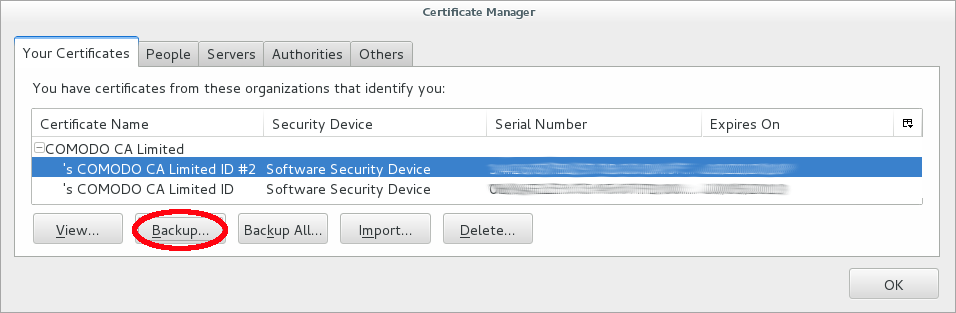
\includegraphics[width=0.7\textwidth]{images/firefox_cert_settings.png}
\item Highlight the line showing your new key.  It will be under the
  name of the CA you chose (e.g. the line under ``COMODO CA Limited''
  if you chose Comodo).
\item %\raisebox{0.6\baselineskip}{\parbox[t]{0.9\textwidth}{%
      %\begin{wrapfigure}{r}{0.7\textwidth}%
      %  \includegraphics[width=0.7\textwidth]{mailapp_firefox_cert_settings.png}
      %\end{wrapfigure}
  Click ``\texttt{Backup...}'' to export the key.
\item Save the file somewhere with a filename of your choice.  It will
  likely be given a \verb|.p12| extension.
\item\label{makebupw} You will be prompted for a password for the
  backup file.  A weak password is fine, because this backup file will
  not be transmitted or retained for long.  You will import it into
  Outlook locally, and then you will delete the backup file.
\item Now your private key must be imported into Outlook.  I'm not
  entirely sure how to do it, but
  \href{https://www.ablebits.com/office-addins-blog/2014/04/11/email-encryption-outlook/}{this
    document} gives the steps for configuring Outlook as needed:\\
  \url{https://www.ablebits.com/office-addins-blog/2014/04/11/email-encryption-outlook/}\\
  Ignore the top of the document because you already have a ``digital
  ID'', and scroll down to ``How to set up your e-mail certificate in
  Outlook''.  This will likely take you close to the place in the
  settings where you can import the key from the backup file.
\item After the key is imported into Outlook, you should delete the
  backup file.  (You can always create a new backup file from Firefox
  if needed).
\end{enumerate}

\subsection{Distribute your S/MIME certificate (aka public key)}
In short: simply send an e-mail to the recipient using Outlook, and sign the message.\\

Detailed explanation: You have a pair of keys (these were created in
section~\ref{catable}).  One is a public key and the other is a
private key.  The public key must be sent to those who will send you
encrypted e-mail.  They will use your public key to encrypt messages
to you.  Your public key is automatically contained in the signature
of all messages you sign.

So to distribute your public key, simply send the other party an
signed e-mail from Outlook.  Encrypting this key distribution message
is optional, but it must be signed.  They can then extract your public
key from your signature.

\section{Prep to send encrypted mail% or verify signatures on received mail
}
Before you can send someone an encrypted message, you need the
recipients S/MIME certificate (public key).  This will normally come
to you when they send you a signed message, at which point you can
extract the certificate.  The certificate must then be associated to
that person in your address book.

\end{document}

% Extra notes for protonmail users:
% 
% 1) click on "SETTINGS" at the top.
% 2) click on "Keys" in the left frame
% 3) click on "Public Key" under the "Download" column
% 4) choose "save file", and save it to a place where you will remember (for the next step)
% 5) compose an e-mail to me, and attach that file you just saved

